% =============================================================================
%                    WEEK 2: NON-COOPERATIVE GAMES (PART II)
% =============================================================================
\section{Week 2: Non-Cooperative Games (Part II)}

% -----------------------------------------------------------------------------
%                              2.1 TOPIC SUMMARY
% -----------------------------------------------------------------------------
\subsection{Topic Summary}

\begin{keybox}[Learning Objectives]
By the end of this week, you will be able to:
\begin{enumerate}
  \item Define the core concepts of non-cooperative game theory, including \textbf{strategy profiles}, \textbf{payoff functions}, and the distinction between cooperative and non-cooperative games.
  \item Formulate real-world scenarios as \textbf{strategic-form (normal-form)} or extensive-form games involving rational, self-interested agents.
  \item Identify and classify various types of strategies: \textbf{pure}, \textbf{mixed}, \textbf{dominant}, and \textbf{best response} strategies.
  \item Analyse game-theoretic models to determine the existence and properties of \textbf{Nash equilibria} (in pure and mixed strategies) and other solution concepts.
  \item Explain and interpret equilibrium behaviour in classical games such as the Prisoner's Dilemma, Matching Pennies, Battle of the Sexes, and coordination games.
  \item Evaluate the potential for and limitations of non-cooperative solutions, including issues of \textbf{uniqueness}, \textbf{multiplicity}, and \textbf{inefficiency} of equilibria.
  \item Demonstrate competency in using mathematical notation and reasoning to represent and solve strategic games.
\end{enumerate}
\end{keybox}

\separator

\subsubsection*{The Big Picture}

This week explores how strategic interactions evolve over time (\textbf{equilibrium dynamics}) and investigates the \textbf{efficiency of equilibria}. We study:

\begin{itemize}
  \item \textbf{Congestion games:} A structured class of large games with concise representation
  \item \textbf{Best-response dynamics:} How agents naturally converge to equilibria
  \item \textbf{Potential functions:} A powerful tool for proving equilibrium existence
  \item \textbf{Price of Anarchy/Stability:} Quantifying the cost of selfish behaviour
\end{itemize}

The central question: \textit{``How inefficient are equilibria compared to socially optimal outcomes?''}

\separator

\subsubsection*{What Examiners Like to Ask}

\begin{itemize}
  \item Define a \textbf{congestion game} formally; specify players, resources, actions, and cost functions.
  \item Given a network graph, compute player costs in different states and identify \textbf{Nash equilibria}.
  \item Explain why best-response dynamics converge in congestion games using \textbf{Rosenthal's potential function}.
  \item Calculate the \textbf{Price of Anarchy} and \textbf{Price of Stability} for given games.
  \item Prove bounds relating social cost to potential function values.
  \item Design games achieving specific PoA/PoS values (e.g., cut games with PoA = 2).
\end{itemize}

\separator

% -----------------------------------------------------------------------------
%                 2.2 OVERVIEW + CORE CONCEPTS + EXTENDED THEORY
% -----------------------------------------------------------------------------
\subsection{Overview + Core Concepts + Extended Theory}

\subsubsection*{Roadmap}
\begin{enumerate}
  \item Large games and representation complexity
  \item Congestion games: formal definition
  \item Network/routing congestion games
  \item Applications of congestion games
  \item Best-response dynamics
  \item Rosenthal's potential function
  \item Potential games and the finite improvement property
  \item Price of Anarchy and Price of Stability
  \item Linear congestion games and tight bounds
\end{enumerate}

\bigseparator

% --- Large Games ---
\subsubsection{Large Games and Representation}

\begin{defbox}[Representation Complexity]
To represent an $n$-player game where each player has $k$ actions in normal form, we need $\mathbf{k^n}$ numbers just to encode the utility functions.

\textbf{Problem:} For even moderately large $k$ and $n$, this is intractable.

\textbf{Solution:} Study games with \textbf{concise structure} that allows compact representation and efficient reasoning.
\end{defbox}

\begin{tipbox}[Exam Tip]
When asked about scalability of game representations, emphasize that normal form requires exponential space in the number of players, motivating structured game classes like congestion games.
\end{tipbox}

\bigseparator

% --- Congestion Games ---
\subsubsection{Congestion Games}

\begin{defbox}[Congestion Game (Formal Definition)]
A \textbf{congestion game} is defined by the tuple $(N, R, (A_i)_{i \in N}, (d_j)_{j \in R})$ where:

\begin{itemize}
  \item $N = \{1, 2, \ldots, n\}$ is the set of \textbf{players}
  \item $R = \{1, 2, \ldots, m\}$ is the set of \textbf{facilities} (or resources)
  \item For each player $i$, $A_i \subseteq 2^R$ is the set of \textbf{actions}, where each action $a_i \in A_i$ is a subset of facilities
  \item For each facility $j \in R$, $d_j : \{0, 1, \ldots, n\} \to \mathbb{R}_{\geq 0}$ is the \textbf{cost (delay) function}
\end{itemize}

\textbf{Key insight:} The cost of a facility depends \textit{only} on how many players use it, not on which specific players.
\end{defbox}

\begin{defbox}[Player Costs in Congestion Games]
Given action profile $a = (a_1, \ldots, a_n)$:

\textbf{Congestion on facility $j$:}
\[
n_j(a) = |\{i : j \in a_i\}|
\]
(number of players using facility $j$)

\textbf{Cost to player $i$:}
\[
c_i(a) = \sum_{j \in a_i} d_j(n_j(a))
\]
(sum of delay costs over all facilities in player $i$'s action)
\end{defbox}

\begin{tipbox}[Exam Tip: Congestion Games vs Normal Form]
Congestion games have \textbf{polynomial representation}: $O(n \cdot |R| + m \cdot n)$ to specify all action sets and delay functions. Compare to $O(k^n)$ for general normal form!
\end{tipbox}

\separator

% --- Network Congestion Games ---
\subsubsection{Network Congestion (Routing) Games}

\begin{defbox}[Network Congestion Game]
A \textbf{network congestion game} (or \textbf{routing game}) is a congestion game where:

\begin{itemize}
  \item There is a directed graph $G = (V, E)$
  \item The resource set $R$ corresponds to the edge set $E$
  \item Each player $i$ has a source-destination pair $(s_i, t_i)$
  \item Player $i$'s action set $A_i$ = set of all directed paths from $s_i$ to $t_i$
\end{itemize}

\textbf{Interpretation:} Each player chooses a route through the network; edge costs depend on congestion.
\end{defbox}

\begin{exbox}[Example: Three-Player Routing Game]
Consider the following network with three players:

\begin{center}
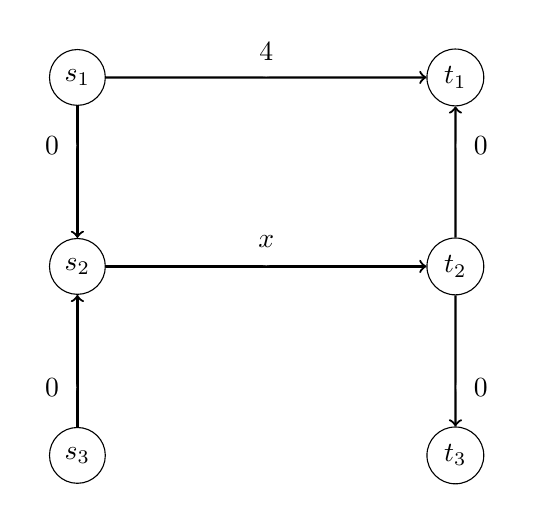
\begin{tikzpicture}[scale=1.2, every node/.style={circle, draw, minimum size=6mm}]
  % Nodes
  \node (s1) at (0, 2) {$s_1$};
  \node (s2) at (0, 0) {$s_2$};
  \node (s3) at (0, -2) {$s_3$};
  \node (t1) at (4, 2) {$t_1$};
  \node (t2) at (4, 0) {$t_2$};
  \node (t3) at (4, -2) {$t_3$};
  
  % Edges with labels
  \draw[->, thick] (s1) -- node[above, draw=none, fill=white] {$4$} (t1);
  \draw[->, thick] (s1) -- node[left, draw=none, fill=white, pos=0.3] {$0$} (s2);
  \draw[->, thick] (s2) -- node[above, draw=none, fill=white] {$x$} (t2);
  \draw[->, thick] (s3) -- node[left, draw=none, fill=white, pos=0.3] {$0$} (s2);
  \draw[->, thick] (t2) -- node[right, draw=none, fill=white, pos=0.7] {$0$} (t1);
  \draw[->, thick] (t2) -- node[right, draw=none, fill=white, pos=0.7] {$0$} (t3);
\end{tikzpicture}
\end{center}

\textbf{Setup:}
\begin{itemize}
  \item Player 1: $s_1 \to t_1$ (two paths available)
  \item Player 2: $s_2 \to t_2$ (one path: direct)
  \item Player 3: $s_3 \to t_3$ (one path: via $s_2, t_2$)
\end{itemize}

\textbf{Edge costs:} Most edges have constant cost; edge $(s_2, t_2)$ has cost $d(x) = x$ (identity function).

\textbf{Player 1's strategies:}
\begin{enumerate}
  \item Direct path: $\{(s_1, t_1)\}$ with constant cost 4
  \item Indirect path: $\{(s_1, s_2), (s_2, t_2), (t_2, t_1)\}$ with cost $0 + x + 0 = x$
\end{enumerate}

\textbf{State A} (Player 1 takes direct route):
\begin{itemize}
  \item Congestion on $(s_2, t_2)$: 2 (Players 2 and 3)
  \item $c_1(A) = 4$, \quad $c_2(A) = 2$, \quad $c_3(A) = 2$
  \item Social cost: $4 + 2 + 2 = 8$
\end{itemize}

\textbf{State B} (Player 1 takes indirect route):
\begin{itemize}
  \item Congestion on $(s_2, t_2)$: 3 (all players)
  \item $c_1(B) = 3$, \quad $c_2(B) = 3$, \quad $c_3(B) = 3$
  \item Social cost: $3 + 3 + 3 = 9$
\end{itemize}

\textbf{Analysis:}
\begin{itemize}
  \item \textbf{Nash Equilibrium:} State B (Player 1 prefers cost 3 over cost 4)
  \item \textbf{Social Optimum:} State A (total cost 8 vs 9)
  \item Selfish behaviour leads to \textbf{inefficient} equilibrium!
\end{itemize}
\end{exbox}

\bigseparator

% --- Applications ---
\subsubsection{Applications of Congestion Games}

Congestion games model decentralised decision-making in shared, congestible environments:

\begin{center}
\renewcommand{\arraystretch}{1.4}
\begin{tabular}{@{} l p{9cm} @{}}
\toprule
\textbf{Domain} & \textbf{Application} \\
\midrule
Traffic \& Transportation & Drivers choose routes to minimise travel time; analysis of road networks, navigation apps, highway design \\
Telecommunications & Data packets select routes/channels; TCP/IP routing, spectrum allocation, cellular load balancing \\
Cloud Computing & Jobs compete for CPUs, memory, bandwidth in data centres \\
Robotics & Multiple robots share warehouse aisles, coordinate movement \\
Smart Grids & Consumers choose when to use electricity; demand response \\
IoT Networks & Devices compete for transmission time, battery, sensors \\
Shared Economy & Ride-hailing, bike-sharing: too many users at one location reduces utility \\
AI/ML Resources & Competing agents select computing resources; federated learning \\
Cybersecurity & Attackers/defenders allocate resources across network surfaces \\
Urban Planning & Citizens choose public resources (parks, hospitals); overuse degrades quality \\
\bottomrule
\end{tabular}
\end{center}

\bigseparator

% --- Best Response Dynamics ---
\subsubsection{Best Response Dynamics}

\begin{defbox}[Best Response Dynamics]
\textbf{Algorithm:}
\begin{enumerate}
  \item Start with an arbitrary action profile $a = (a_1, \ldots, a_n)$
  \item While $\exists$ player $i$ who can decrease their cost by switching:
  \begin{itemize}
    \item Player $i$ switches to a \textbf{best response} (or any improving response)
  \end{itemize}
  \item If/when the process halts, return the current profile
\end{enumerate}

\textbf{Key observation:} If best-response dynamics halts, the output is a \textbf{pure Nash equilibrium} (by definition: no player has a profitable deviation).
\end{defbox}

\begin{exbox}[Example: Best Response Dynamics in a Routing Game]
Consider two players (Red and Blue) travelling from $S$ to $T$:

\begin{center}
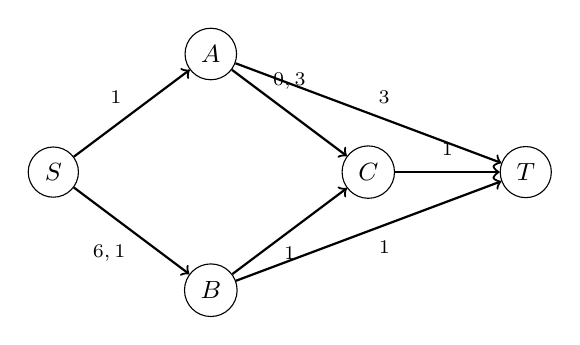
\begin{tikzpicture}[scale=1.0, every node/.style={circle, draw, minimum size=5mm, font=\small}]
  % Main nodes
  \node (S) at (0, 0) {$S$};
  \node (A) at (2, 1.5) {$A$};
  \node (B) at (2, -1.5) {$B$};
  \node (C) at (4, 0) {$C$};
  \node (T) at (6, 0) {$T$};
  
  % Edges - upper path
  \draw[->, thick] (S) -- node[above left, draw=none, font=\scriptsize] {$1$} (A);
  \draw[->, thick] (A) -- node[above, draw=none, font=\scriptsize] {$0,3$} (C);
  \draw[->, thick] (A) -- node[above right, draw=none, font=\scriptsize] {$3$} (T);
  
  % Edges - lower path  
  \draw[->, thick] (S) -- node[below left, draw=none, font=\scriptsize] {$6,1$} (B);
  \draw[->, thick] (B) -- node[below, draw=none, font=\scriptsize] {$1$} (C);
  \draw[->, thick] (B) -- node[below right, draw=none, font=\scriptsize] {$1$} (T);
  
  % Central edge
  \draw[->, thick] (C) -- node[above, draw=none, font=\scriptsize] {$1$} (T);
\end{tikzpicture}
\end{center}

Edge labels show cost for 1 user, or (cost for 1, cost for 2) if congestion-dependent.

\textbf{Initial state:} Red takes upper path $S \to A \to T$, Blue takes lower path $S \to B \to T$.
\begin{itemize}
  \item Red's cost: $1 + 0 + 3 = 4$
  \item Blue's cost: $6 + 1 = 7$
\end{itemize}

\textbf{Round 1 (Red deviates):} Red switches to $S \to A \to C \to T$ (cost: $1 + 0 + 1 = 2 < 4$).

\textbf{Round 2 (Blue deviates):} Blue switches to $S \to B \to C \to T$ (cost: $1 + 1 + 3 = 5 < 7$).
\begin{itemize}
  \item Now both use edge $(C, T)$, so Red's cost becomes $1 + 0 + 3 = 4$
\end{itemize}

\textbf{Round 3 (Red deviates):} Red switches back to $S \to A \to T$ (cost: $1 + 0 + 3 = 4$). Same cost, but let's say no strict improvement.

\textbf{Equilibrium reached:} Red on $S \to A \to T$ (cost 4), Blue on $S \to B \to C \to T$ (cost 3).

Neither player can improve $\Rightarrow$ \textbf{Nash Equilibrium}.
\end{exbox}

\begin{defbox}[Question: Do Best Response Dynamics Always Converge?]
\textbf{No!} Consider Matching Pennies:
\begin{center}
\renewcommand{\arraystretch}{1.2}
\begin{tabular}{@{} c | c c @{}}
 & H & T \\
\midrule
H & $1, -1$ & $-1, 1$ \\
T & $-1, 1$ & $1, -1$ \\
\end{tabular}
\end{center}

From any profile, some player has a profitable deviation $\Rightarrow$ \textbf{cycle forever}.

\textbf{But:} For \textbf{congestion games}, best-response dynamics \textit{always} converges!
\end{defbox}

\bigseparator

% --- Rosenthal's Theorem ---
\subsubsection{Rosenthal's Potential Function}

\begin{thmbox}[Theorem (Rosenthal, 1973)]
For every congestion game, every sequence of improvement steps is \textbf{finite}.

This property is called the \textbf{Finite Improvement Property (FIP)}.
\end{thmbox}

\begin{defbox}[Corollary]
Every congestion game has at least one \textbf{pure strategy Nash equilibrium}.
\end{defbox}

\begin{defbox}[Rosenthal's Potential Function]
For any action profile $a$, define:
\[
\boxed{\Phi(a) = \sum_{j=1}^{m} \sum_{k=1}^{n_j(a)} d_j(k)}
\]

where $n_j(a)$ is the number of players using facility $j$ under profile $a$.

\textbf{Interpretation:} Sum of ``cumulative delay costs'' over all facilities, summing delay values from 1 up to the actual congestion level.
\end{defbox}

\begin{thmbox}[Proof of Rosenthal's Theorem]
Consider a single improvement step where player $i$ switches from action $a_i$ to $b_i$.

\textbf{Change in player $i$'s cost:}
\[
\Delta c_i = c_i(b_i, a_{-i}) - c_i(a_i, a_{-i}) = \sum_{j \in b_i \setminus a_i} d_j(n_j(a) + 1) - \sum_{j \in a_i \setminus b_i} d_j(n_j(a))
\]

Since this is an improvement step: $\Delta c_i < 0$.

\textbf{Change in potential:}
\[
\Delta \Phi = \Phi(b_i, a_{-i}) - \Phi(a_i, a_{-i}) = \sum_{j \in b_i \setminus a_i} d_j(n_j(a) + 1) - \sum_{j \in a_i \setminus b_i} d_j(n_j(a))
\]

\textbf{Key observation:} $\Delta \Phi = \Delta c_i < 0$.

Since $\Phi$ takes finitely many values (finitely many profiles) and \textbf{strictly decreases} at each improvement step, the process must terminate. \qed
\end{thmbox}

\begin{tipbox}[Exam Tip: The Potential Function Trick]
The key insight is that the potential function exactly tracks individual cost changes:
\begin{itemize}
  \item Facilities in $b_i \setminus a_i$: player joins, congestion increases by 1
  \item Facilities in $a_i \setminus b_i$: player leaves, congestion decreases by 1
  \item Facilities in $a_i \cap b_i$: no change to congestion
\end{itemize}
Both the player's cost change and the potential change depend only on the ``boundary'' facilities.
\end{tipbox}

\separator

% --- Potential Games ---
\subsubsection{Potential Games}

\begin{defbox}[Exact Potential Game]
A game $(N, (A_i)_{i \in N}, (U_i)_{i \in N})$ is an \textbf{exact potential game} if there exists a function $\Phi : A \to \mathbb{R}$ such that for every profile $a$, player $i$, and alternative action $a'_i$:
\[
U_i(a'_i, a_{-i}) - U_i(a_i, a_{-i}) = \Phi(a'_i, a_{-i}) - \Phi(a_i, a_{-i})
\]

The function $\Phi$ is called the \textbf{exact potential function}.

\textbf{Key insight:} The change in any player's utility equals the change in the potential function.
\end{defbox}

\begin{defbox}[Properties of Potential Games]
\begin{itemize}
  \item Every \textbf{exact potential game} has the Finite Improvement Property
  \item Every exact potential game has at least one \textbf{pure strategy Nash equilibrium}
  \item Local minima of $\Phi$ correspond to pure NE (for cost-minimisation games)
  \item \textbf{Congestion games are exact potential games} (Rosenthal's potential)
\end{itemize}
\end{defbox}

\begin{tipbox}[Exam Tip: Potential Games]
To show a game is a potential game:
\begin{enumerate}
  \item Propose a potential function $\Phi$
  \item Show that for any unilateral deviation, $\Delta U_i = \Delta \Phi$
\end{enumerate}
This immediately implies existence of pure NE and convergence of best-response dynamics.
\end{tipbox}

\bigseparator

% --- Price of Anarchy/Stability ---
\subsubsection{Price of Anarchy and Price of Stability}

\begin{defbox}[Motivation: Inefficiency of Equilibria]
Selfish behaviour can lead to socially suboptimal outcomes. We quantify this inefficiency by comparing equilibria to optimal solutions.
\end{defbox}

\begin{exbox}[Pigou's Example]
\begin{center}
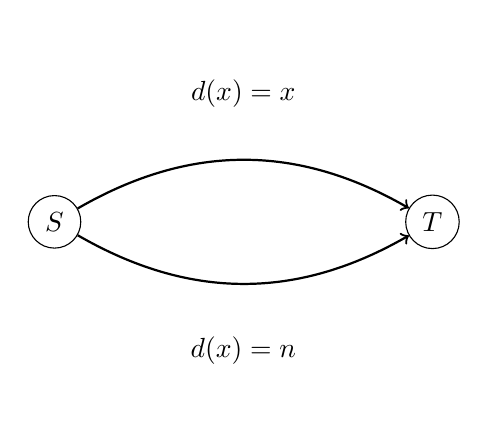
\begin{tikzpicture}[scale=1.2, every node/.style={circle, draw, minimum size=6mm}]
  \node (S) at (0, 0) {$S$};
  \node (T) at (4, 0) {$T$};
  
  % Upper edge (congestion-dependent)
  \draw[->, thick, bend left=30] (S) to node[above, draw=none] {$d(x) = x$} (T);
  
  % Lower edge (constant)
  \draw[->, thick, bend right=30] (S) to node[below, draw=none] {$d(x) = n$} (T);
\end{tikzpicture}
\end{center}

\textbf{Setup:} $n$ players travel from $S$ to $T$. Upper edge has cost = congestion; lower edge has constant cost $n$.

\textbf{Selfish outcome:} All players use the upper edge!
\begin{itemize}
  \item If any player is on the lower edge (cost $n$), upper edge has $< n$ players, so cost $< n$
  \item Lower-edge player is ``envious'' and would switch
  \item \textbf{Equilibrium:} All on upper edge, each pays $n$, total cost = $n^2$
\end{itemize}

\textbf{Social optimum:} Split traffic equally
\begin{itemize}
  \item $n/2$ on upper (each pays $n/2$), $n/2$ on lower (each pays $n$)
  \item Total cost = $\frac{n}{2} \cdot \frac{n}{2} + \frac{n}{2} \cdot n = \frac{n^2}{4} + \frac{n^2}{2} = \frac{3n^2}{4}$
\end{itemize}

\textbf{Efficiency loss:} $\displaystyle\frac{n^2}{3n^2/4} = \frac{4}{3}$
\end{exbox}

\begin{defbox}[Price of Anarchy and Price of Stability]
Given an optimisation objective (minimise cost or maximise welfare):

\textbf{Price of Anarchy (PoA):}
\[
\text{PoA} = \frac{\text{value of worst Nash equilibrium}}{\text{value of optimal solution}}
\]

\textbf{Price of Stability (PoS):}
\[
\text{PoS} = \frac{\text{value of best Nash equilibrium}}{\text{value of optimal solution}}
\]

\textbf{Convention:} For minimisation problems, PoA, PoS $\geq 1$. For maximisation, invert the fraction so PoA, PoS $\geq 1$.

\textbf{Interpretation:}
\begin{itemize}
  \item $\text{PoA} = 1$: worst equilibrium is optimal (rare)
  \item $\text{PoS} = 1$: at least one optimal equilibrium exists
  \item Large PoA: selfish behaviour can be very costly
\end{itemize}
\end{defbox}

\begin{exbox}[Prisoner's Dilemma: PoA and PoS]
\begin{center}
\renewcommand{\arraystretch}{1.2}
\begin{tabular}{@{} c | c c @{}}
 & C & D \\
\midrule
C & $10, 10$ & $0, 12$ \\
D & $12, 0$ & $1, 1$ \\
\end{tabular}
\end{center}

\textbf{Objective:} Maximise social welfare (sum of utilities).

\begin{itemize}
  \item \textbf{Unique NE:} $(D, D)$ with welfare $1 + 1 = 2$
  \item \textbf{Social optimum:} $(C, C)$ with welfare $10 + 10 = 20$
\end{itemize}

\[
\text{PoA} = \text{PoS} = \frac{20}{2} = 10
\]

\textbf{Interpretation:} Selfish behaviour loses a factor of 10 in efficiency!
\end{exbox}

\begin{exbox}[Battle of the Sexes: PoA and PoS]
\begin{center}
\renewcommand{\arraystretch}{1.2}
\begin{tabular}{@{} c | c c @{}}
 & Theatre & Football \\
\midrule
Theatre & $2, 1$ & $0, 0$ \\
Football & $0, 0$ & $1, 2$ \\
\end{tabular}
\end{center}

\textbf{Objective:} Maximise social welfare.

\begin{itemize}
  \item \textbf{NE 1:} (Theatre, Theatre) with welfare $2 + 1 = 3$
  \item \textbf{NE 2:} (Football, Football) with welfare $1 + 2 = 4$
  \item \textbf{Social optimum:} welfare $4$ (achieved by NE 2)
\end{itemize}

\[
\text{PoS} = \frac{4}{4} = 1, \quad \text{PoA} = \frac{4}{3}
\]

\textbf{Interpretation:} Best equilibrium is optimal, but coordination failure can cost $\frac{1}{3}$ of optimal welfare.
\end{exbox}

\begin{exbox}[Three-Player Routing Game: PoA and PoS]
Returning to our earlier example:
\begin{itemize}
  \item \textbf{Unique NE:} State B (all use shared edge), social cost = 9
  \item \textbf{Social optimum:} State A, social cost = 8
\end{itemize}

\[
\text{PoA} = \text{PoS} = \frac{9}{8}
\]
\end{exbox}

\bigseparator

% --- Linear Congestion Games ---
\subsubsection{Linear Congestion Games}

\begin{defbox}[Linear Congestion Game]
A congestion game is \textbf{linear} if all cost functions have the form:
\[
d_j(x) = a_j \cdot x + b_j
\]
where $a_j \geq 0$ and $b_j \geq 0$ are constants.

\textbf{Special case:} If $b_j = 0$ for all $j$, the game has \textbf{identity cost functions}.
\end{defbox}

\begin{thmbox}[Theorem (Christodoulou and Koutsoupias, 2005)]
For any congestion game with \textbf{linear cost functions}, the Price of Anarchy is at most $\mathbf{2.5}$.
\end{thmbox}

\begin{thmbox}[Theorem (Christodoulou and Koutsoupias, 2005)]
There exist linear congestion games with 3 or more players where the Price of Anarchy equals $\mathbf{2.5}$ (tight bound).
\end{thmbox}

\begin{exbox}[Tight PoA = 2.5 Example (4 Players)]
\begin{center}
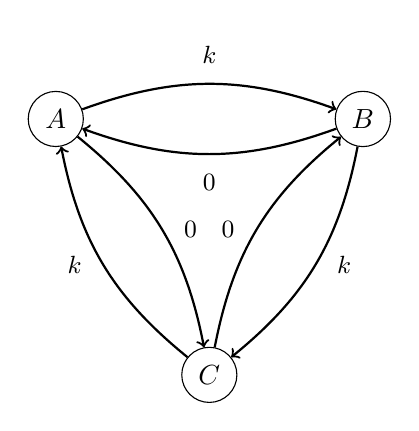
\begin{tikzpicture}[scale=1.3, every node/.style={circle, draw, minimum size=7mm}]
  \node (A) at (0, 0) {$A$};
  \node (B) at (3, 0) {$B$};
  \node (C) at (1.5, -2.5) {$C$};
  
  % Direct edges (cost k each)
  \draw[->, thick] (A) to[bend left=20] node[above, draw=none, font=\small] {$k$} (B);
  \draw[->, thick] (B) to[bend left=20] node[right, draw=none, font=\small] {$k$} (C);
  \draw[->, thick] (C) to[bend left=20] node[left, draw=none, font=\small] {$k$} (A);
  
  % Reverse edges (cost 0 each)
  \draw[->, thick] (B) to[bend left=20] node[below, draw=none, font=\small] {$0$} (A);
  \draw[->, thick] (C) to[bend left=20] node[left, draw=none, font=\small] {$0$} (B);
  \draw[->, thick] (A) to[bend left=20] node[right, draw=none, font=\small] {$0$} (C);
\end{tikzpicture}
\end{center}

\textbf{Players and destinations:}
\begin{itemize}
  \item Player 1: $A \to B$
  \item Player 2: $A \to C$
  \item Player 3: $B \to C$
  \item Player 4: $C \to B$
\end{itemize}

\textbf{Edge costs:} $d_j(x) = k \cdot x$ for ``clockwise'' edges; $d_j(x) = 0$ for ``counter-clockwise'' edges.

\textbf{Optimal solution:} Each player takes the direct path (cost $k$ each).
\begin{itemize}
  \item Total cost: $k + k + k + k = 4k$
  \item This is also a NE (any deviation uses at least one cost-$k$ edge)
\end{itemize}

\textbf{Worst NE:} Players take longer paths:
\begin{itemize}
  \item Player 1: $A \to C \to B$ (cost $0 + 2k = 2k$, but with congestion...)
  \item Player 2: $A \to B \to C$ (cost $2k + k$...)
  \item Player 3: $B \to A \to C$ (cost...)
  \item Player 4: $C \to A \to B$ (cost...)
\end{itemize}

After computing congestion effects:
\begin{itemize}
  \item Players 1 and 2: cost $2k + k = 3k$ each (2 players on each edge they use)
  \item Players 3 and 4: cost $0 + 2k = 2k$ each
  \item Total: $3k + 3k + 2k + 2k = 10k$
\end{itemize}

\textbf{Price of Anarchy:} $\displaystyle\frac{10k}{4k} = \frac{10}{4} = 2.5$
\end{exbox}

\bigseparator

% --- Bounds on Potential vs Social Cost ---
\subsubsection{Relating Potential Function to Social Cost}

\begin{thmbox}[Lemma: Potential Bounds for Linear Congestion Games]
For any linear congestion game and any strategy profile $s$:
\[
\frac{1}{2} \cdot SC(s) \leq \Phi(s) \leq SC(s)
\]
where $SC(s) = \sum_{i} c_i(s)$ is the social cost.
\end{thmbox}

\begin{thmbox}[Proof Sketch]
For linear costs $d_j(x) = a_j \cdot x + b_j$:

\textbf{Social cost contribution from resource $j$:}
\[
SC_j = n_j(s) \cdot d_j(n_j(s)) = n_j(s) \cdot (a_j \cdot n_j(s) + b_j) = a_j \cdot n_j(s)^2 + b_j \cdot n_j(s)
\]

\textbf{Potential contribution from resource $j$:}
\[
\Phi_j = \sum_{k=1}^{n_j(s)} (a_j \cdot k + b_j) = a_j \cdot \frac{n_j(s)(n_j(s)+1)}{2} + b_j \cdot n_j(s)
\]

Comparing:
\begin{itemize}
  \item $\Phi_j \leq SC_j$ because $\frac{n(n+1)}{2} \leq n^2$ (equality when $n=1$)
  \item $\Phi_j \geq \frac{1}{2} SC_j$ because $\frac{n(n+1)}{2} \geq \frac{n^2}{2}$
\end{itemize}
\end{thmbox}

\begin{tipbox}[Exam Tip: Using Potential to Bound PoS]
If a game has potential function $\Phi$ with $\alpha \cdot SC(s) \leq \Phi(s) \leq \beta \cdot SC(s)$, then:
\[
\text{PoS} \leq \frac{\beta}{\alpha}
\]
Because the best NE minimises $\Phi$, and the optimal solution minimises $SC$.
\end{tipbox}

\bigseparator

% --- Worked Examples ---
\subsubsection{Worked Examples from Exercises}

\begin{exbox}[Exercise 1: Finding NE in a Network Congestion Game]
\begin{center}
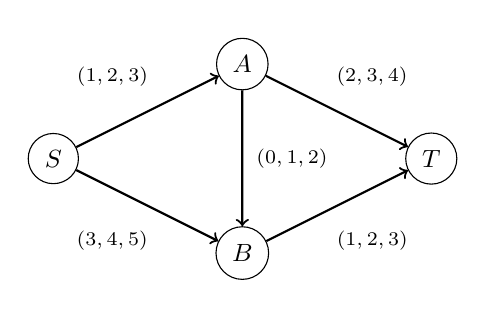
\begin{tikzpicture}[scale=1.2, every node/.style={circle, draw, minimum size=6mm, font=\small}]
  \node (S) at (0, 0) {$S$};
  \node (A) at (2, 1) {$A$};
  \node (B) at (2, -1) {$B$};
  \node (T) at (4, 0) {$T$};
  
  \draw[->, thick] (S) -- node[above left, draw=none, font=\scriptsize] {$(1,2,3)$} (A);
  \draw[->, thick] (S) -- node[below left, draw=none, font=\scriptsize] {$(3,4,5)$} (B);
  \draw[->, thick] (A) -- node[above right, draw=none, font=\scriptsize] {$(2,3,4)$} (T);
  \draw[->, thick] (B) -- node[below right, draw=none, font=\scriptsize] {$(1,2,3)$} (T);
  \draw[->, thick] (A) -- node[right, draw=none, font=\scriptsize] {$(0,1,2)$} (B);
\end{tikzpicture}
\end{center}

\textbf{Setup:} Three players, each travels $S \to T$. Edge labels $(c_1, c_2, c_3)$ show cost when 1, 2, or 3 players use that edge.

\textbf{Available paths:}
\begin{enumerate}
  \item $S \to A \to T$
  \item $S \to B \to T$
  \item $S \to A \to B \to T$
\end{enumerate}

\textbf{Solution approach:}
\begin{enumerate}
  \item List all strategy profiles (there are $3^3 = 27$, but symmetry helps)
  \item For each profile, compute player costs
  \item Check if any player can improve by switching
\end{enumerate}

\textbf{Candidate NE:} All players take $S \to A \to T$.
\begin{itemize}
  \item Edge $(S,A)$: 3 players, cost = 3 each
  \item Edge $(A,T)$: 3 players, cost = 4 each
  \item Total cost per player: $3 + 4 = 7$
\end{itemize}

\textbf{Check deviations:}
\begin{itemize}
  \item Switch to $S \to B \to T$: cost = $3 + 1 = 4 < 7$ \checkmark Profitable!
\end{itemize}

This is \textbf{not} a NE. Continue checking other profiles...

\textbf{NE:} (Found by systematic enumeration) Two players on $S \to A \to T$, one on $S \to B \to T$.
\end{exbox}

\begin{exbox}[Exercise 2: Potential Function Bounds]
\textbf{Claim:} For linear congestion games, $\frac{1}{2} SC(s) \leq \Phi(s) \leq SC(s)$.

\textbf{Proof:} For each resource $j$ with $n_j$ users and cost $d_j(x) = a_j x + b_j$:

Social cost contribution: $SC_j = n_j \cdot d_j(n_j) = a_j n_j^2 + b_j n_j$

Potential contribution: 
\[
\Phi_j = \sum_{k=1}^{n_j} (a_j k + b_j) = a_j \cdot \frac{n_j(n_j+1)}{2} + b_j n_j
\]

\textbf{Upper bound:} $\frac{n_j(n_j+1)}{2} \leq n_j^2$ (since $n_j+1 \leq 2n_j$ for $n_j \geq 1$).

\textbf{Lower bound:} $\frac{n_j(n_j+1)}{2} = \frac{n_j^2}{2} + \frac{n_j}{2} \geq \frac{n_j^2}{2}$.

Summing over all resources gives the result. \qed
\end{exbox}

\begin{exbox}[Exercise 3: PoS Bound Using Potential]
\textbf{Claim:} If no resource is used by more than $\lambda$ players, then $\text{PoS} \leq \lambda$.

\textbf{Proof:} Let $s^*$ be the optimal profile and $\hat{s}$ be the best NE (minimises $\Phi$).

Since NE minimises potential among all NE, and $\Phi$ strictly decreases along improvement paths:
\[
\Phi(\hat{s}) \leq \Phi(s^*)
\]

Using the bounds:
\[
\frac{1}{\lambda} SC(\hat{s}) \leq \Phi(\hat{s}) \leq \Phi(s^*) \leq SC(s^*)
\]

(The first inequality uses that with at most $\lambda$ users, $\Phi_j \geq \frac{1}{\lambda} SC_j$.)

Therefore: $SC(\hat{s}) \leq \lambda \cdot SC(s^*)$, so $\text{PoS} \leq \lambda$. \qed
\end{exbox}

\begin{exbox}[Exercise 4: Cut Games]
\textbf{Definition:} Given graph $G = (V, E)$ with edge weights $w_e$:
\begin{itemize}
  \item Each player $i$ controls vertex $v_i$
  \item Strategy: place $v_i$ in LEFT or RIGHT
  \item Utility: sum of weights of edges incident to $v_i$ that cross the cut
\end{itemize}

\textbf{(a) Design a cut game with PoA = 2:}

\begin{center}
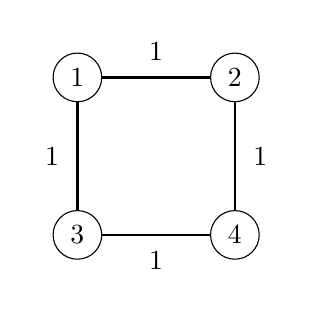
\begin{tikzpicture}[scale=1.0, every node/.style={circle, draw, minimum size=6mm}]
  \node (1) at (0, 1) {1};
  \node (2) at (2, 1) {2};
  \node (3) at (0, -1) {3};
  \node (4) at (2, -1) {4};
  
  \draw[thick] (1) -- node[above, draw=none] {$1$} (2);
  \draw[thick] (3) -- node[below, draw=none] {$1$} (4);
  \draw[thick] (1) -- node[left, draw=none] {$1$} (3);
  \draw[thick] (2) -- node[right, draw=none] {$1$} (4);
\end{tikzpicture}
\end{center}

\textbf{Optimal:} Diagonal cut (vertices 1,4 vs 2,3) cuts all 4 edges. Total utility = 8.

\textbf{Worst NE:} Horizontal cut (vertices 1,2 vs 3,4) cuts 2 edges. Total utility = 4.

$\text{PoA} = \frac{8}{4} = 2$.

\textbf{(b) Prove PoA $\leq 2$:}

In any NE, each player must have at least half their adjacent edge weight in the cut (otherwise switching sides would be profitable).

For player $i$: $u_i \geq \frac{1}{2} \sum_{e \ni v_i} w_e$.

Summing: $\sum_i u_i \geq \frac{1}{2} \sum_i \sum_{e \ni v_i} w_e = \sum_e w_e$ (each edge counted twice).

Optimal welfare $\leq 2 \sum_e w_e$ (at most, each edge crosses the cut, counted for both endpoints).

Therefore: NE welfare $\geq \frac{1}{2}$ optimal $\Rightarrow$ PoA $\leq 2$. \qed
\end{exbox}

\bigseparator

% --- Summary Table ---
\subsubsection{Summary: Key Concepts}

\begin{center}
\renewcommand{\arraystretch}{1.4}
\begin{tabular}{@{} l p{9.5cm} @{}}
\toprule
\textbf{Concept} & \textbf{Key Points} \\
\midrule
Congestion Game & Players choose subsets of resources; cost depends on congestion only \\
Network Congestion Game & Resources are edges; actions are source-to-destination paths \\
Best Response Dynamics & Players iteratively improve; converges in congestion games \\
Rosenthal's Potential & $\Phi(a) = \sum_j \sum_{k=1}^{n_j(a)} d_j(k)$; decreases with each improvement \\
Finite Improvement Property & Every improvement sequence is finite $\Rightarrow$ pure NE exists \\
Price of Anarchy & Worst NE / Optimal (measures cost of selfishness) \\
Price of Stability & Best NE / Optimal (measures cost of decentralisation) \\
Linear Congestion Games & PoA $\leq 2.5$; this bound is tight \\
\bottomrule
\end{tabular}
\end{center}
